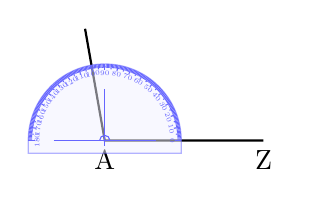
\begin{tikzpicture}[rotate=0,scale=0.18]
\coordinate (A) at (0,0);
\coordinate (Z) at (11.2,0);

\draw [thick](Z) node [below]{Z}--(A) node [below]{A}--([turn]-80:8);


%début du rapporteur
\def \CharSize {0.8};
\def \BulletSize {1};

    %Définition de l 'angle de rotation du rapporteur
\def \Rotation {0} 
    %Couleur des élèments du rapporteur (sauf le remplissage)
\def \RapColor {blue!60}


\begin{scope}[scale=1.8,rotate=\Rotation,every node/.style={scale=0.5}]
    % contours du rapporteur
    \draw[color=\RapColor, fill =blue!5, opacity=0.5] (-3,0) arc(180:0:3)--(3,-0.5)--(-3,-0.5)--cycle;	%Dont couleur de remplissage
    \draw[color=\RapColor] (-2,0)--(2,0);
    \draw[color=\RapColor] (0,-0.2)--(0,2);
    % graduation externe 1 degrés
    \foreach \a in {0,1,...,180}{\draw[color=\RapColor] (\a:3)--(\a:2.85);}
    % graduation externe 5 degrés
    \foreach \a in {0,5,...,180}{\draw[color=\RapColor] (\a:2.85)--(\a:2.8);}
 
    % double graduation
   \foreach \a/\b in {%
        0/-90,10/-80,20/-70,30/-60,40/-50,50/-40,%
        60/-30,70/-20,80/-10,90/0,100/10,110/20,%
        120/30,130/40,140/50,150/60,160/70,170/80,180/90%
    }{
    % graduation externe 10 degrés
    \draw[color=\RapColor] (\a:2.80)--(\a:2.75) 
    node[font=\tiny, rotate=\b+\Rotation] (\a) at (\a:2.65){\a};
 
    % graduation interne 10 degrés
 %   \draw[color=\RapColor] (\a:2.5)--(\a:2.45)
%	node[thin,font=\tiny, rotate=-\b+\Rotation] (\a) at (180-\a:2.3){\a}; 
}
 
    % demi-cercle intérieur
%    \draw[color=\RapColor](-2.5,0) arc(180:0:2.5);

    %demi-cercle à l'origine
    \draw[color=\RapColor](-0.2,0) arc(180:0:0.2);
\end{scope}
%fin du rapporteur


\end{tikzpicture}
 
